\section{Estudo com Redes Neuronais}
Sendo que o pressuposto das Redes Neuronais é que tenham um bom desempenho, em termos da qualidade da prestação de modelos treinados usando o mesmo, foi a primeira abordagem que decidimos dar ao problema.

\subsection{Estrutura usada}
Apesar do \textit{dataset} ter dimensões consideráveis para o \textit{hardware} disponível, consideramos que este problema consegue ser resolvido com uma rede neuronal "normal". O uso de uma rede convolucional neste problema acaba por ser evitado, pois na fase de pré-processamento existiram métodos de selecção de \textit{features} suficientes para o modelo ter uma performance boa, não sendo necessário que o modelo tenha a responsabilidade de fazer a procura de \textit{features}.
Então após a experimentação de alguns valores relativos ao número de neurónios e número de \textit{hidden layers} consideramos uma rede neuronal com as seguintes características:

Input \textrightarrow{} 200 Neurónios \textrightarrow{} 100 Neurónios \textrightarrow{} Output

Os valores dos hiperparâmetros usado foram:
\begin{itemize}
    \item \textbf{Número de \textit{features} (termos do vocabulário)}: 600
    \item \textbf{Número de \textit{epochs}}: 200
    \item \textbf{\textit{Batch size}}: 500
    \item \textbf{\textit{Activation function}}:
        \begin{itemize}
            \item \textbf{\textit{Hidden Layers}}: \textit{Relu} \cite{relu_function}
            \item \textbf{\textit{Output Layer}}: \textit{Softmax} \cite{softmax_function}
        \end{itemize}
    \item \textbf{\textit{Optimizer}}: \textit{Adam} \cite{adam_optimizer}
    \item \textbf{\textit{Loss function}}: \textit{Categorical crossentropy} \cite{categorical_crossentropy_optimizer}
\end{itemize}


Desde o inicio da implementação deste modelo que foi usado o processo de treino-validação utilizando o \textbf{\textit{K-Fold Cross validation}}. Este método tem um parâmetro \textbf{\textit{k}} que define o número de divisões que o conjunto será sujeito, cada porção segmentada é intitulada de \textit{fold}. No processo de treino todos os \textit{folds} são usados para teste uma vez, sendo que os outros restantes \textit{k-1} \textit{folds} são usados para o processo de treino. Neste estudo, o valor de \textit{k} definindo foi 5 (\textbf{\textit{K\textunderscore{fold}} com 5 \textit{splits}}).
Ainda foi adicionado um \textit{callback} de \textit{Early Stopping} com objectivo de suspender o treino quando o parâmetro a ser monitorizado (neste caso o \textit{validation accuracy}) para de melhorar.


\subsection{Resultados obtidos}

Após as condições definidas anteriormente decidimos então testar a performance do modelo. 
Obtivemos os seguintes valores de \textit{accuracy}, após retreino do modelo (com todos os dados de treino e \textit{cross validation}):

\begin{itemize}
        \item \textbf{\textit{Train Score}}: 0.82
        \item \textbf{\textit{Test Score}}: 0.71
\end{itemize}


Como se pode observar pelos resultados e pelo gráfico \ref{diagram:accuracy_retrain}, o modelo tem tendência a realizar o fenómeno de \textit{overfit}, pelo que as próximas subsecções têm como objectivo explicar os mecanismos usados para evitar este fenómeno. Apenas de salientar que devido ao \textit{callback} de  \textit{early stopping}, o treino é parado, pois a \textit{accuracy} do conjunto de validação não aumenta, o que acaba por evitar uma maximização do fenómeno de \textit{overfit}.


\begin{figure}[t]
\begin{center}
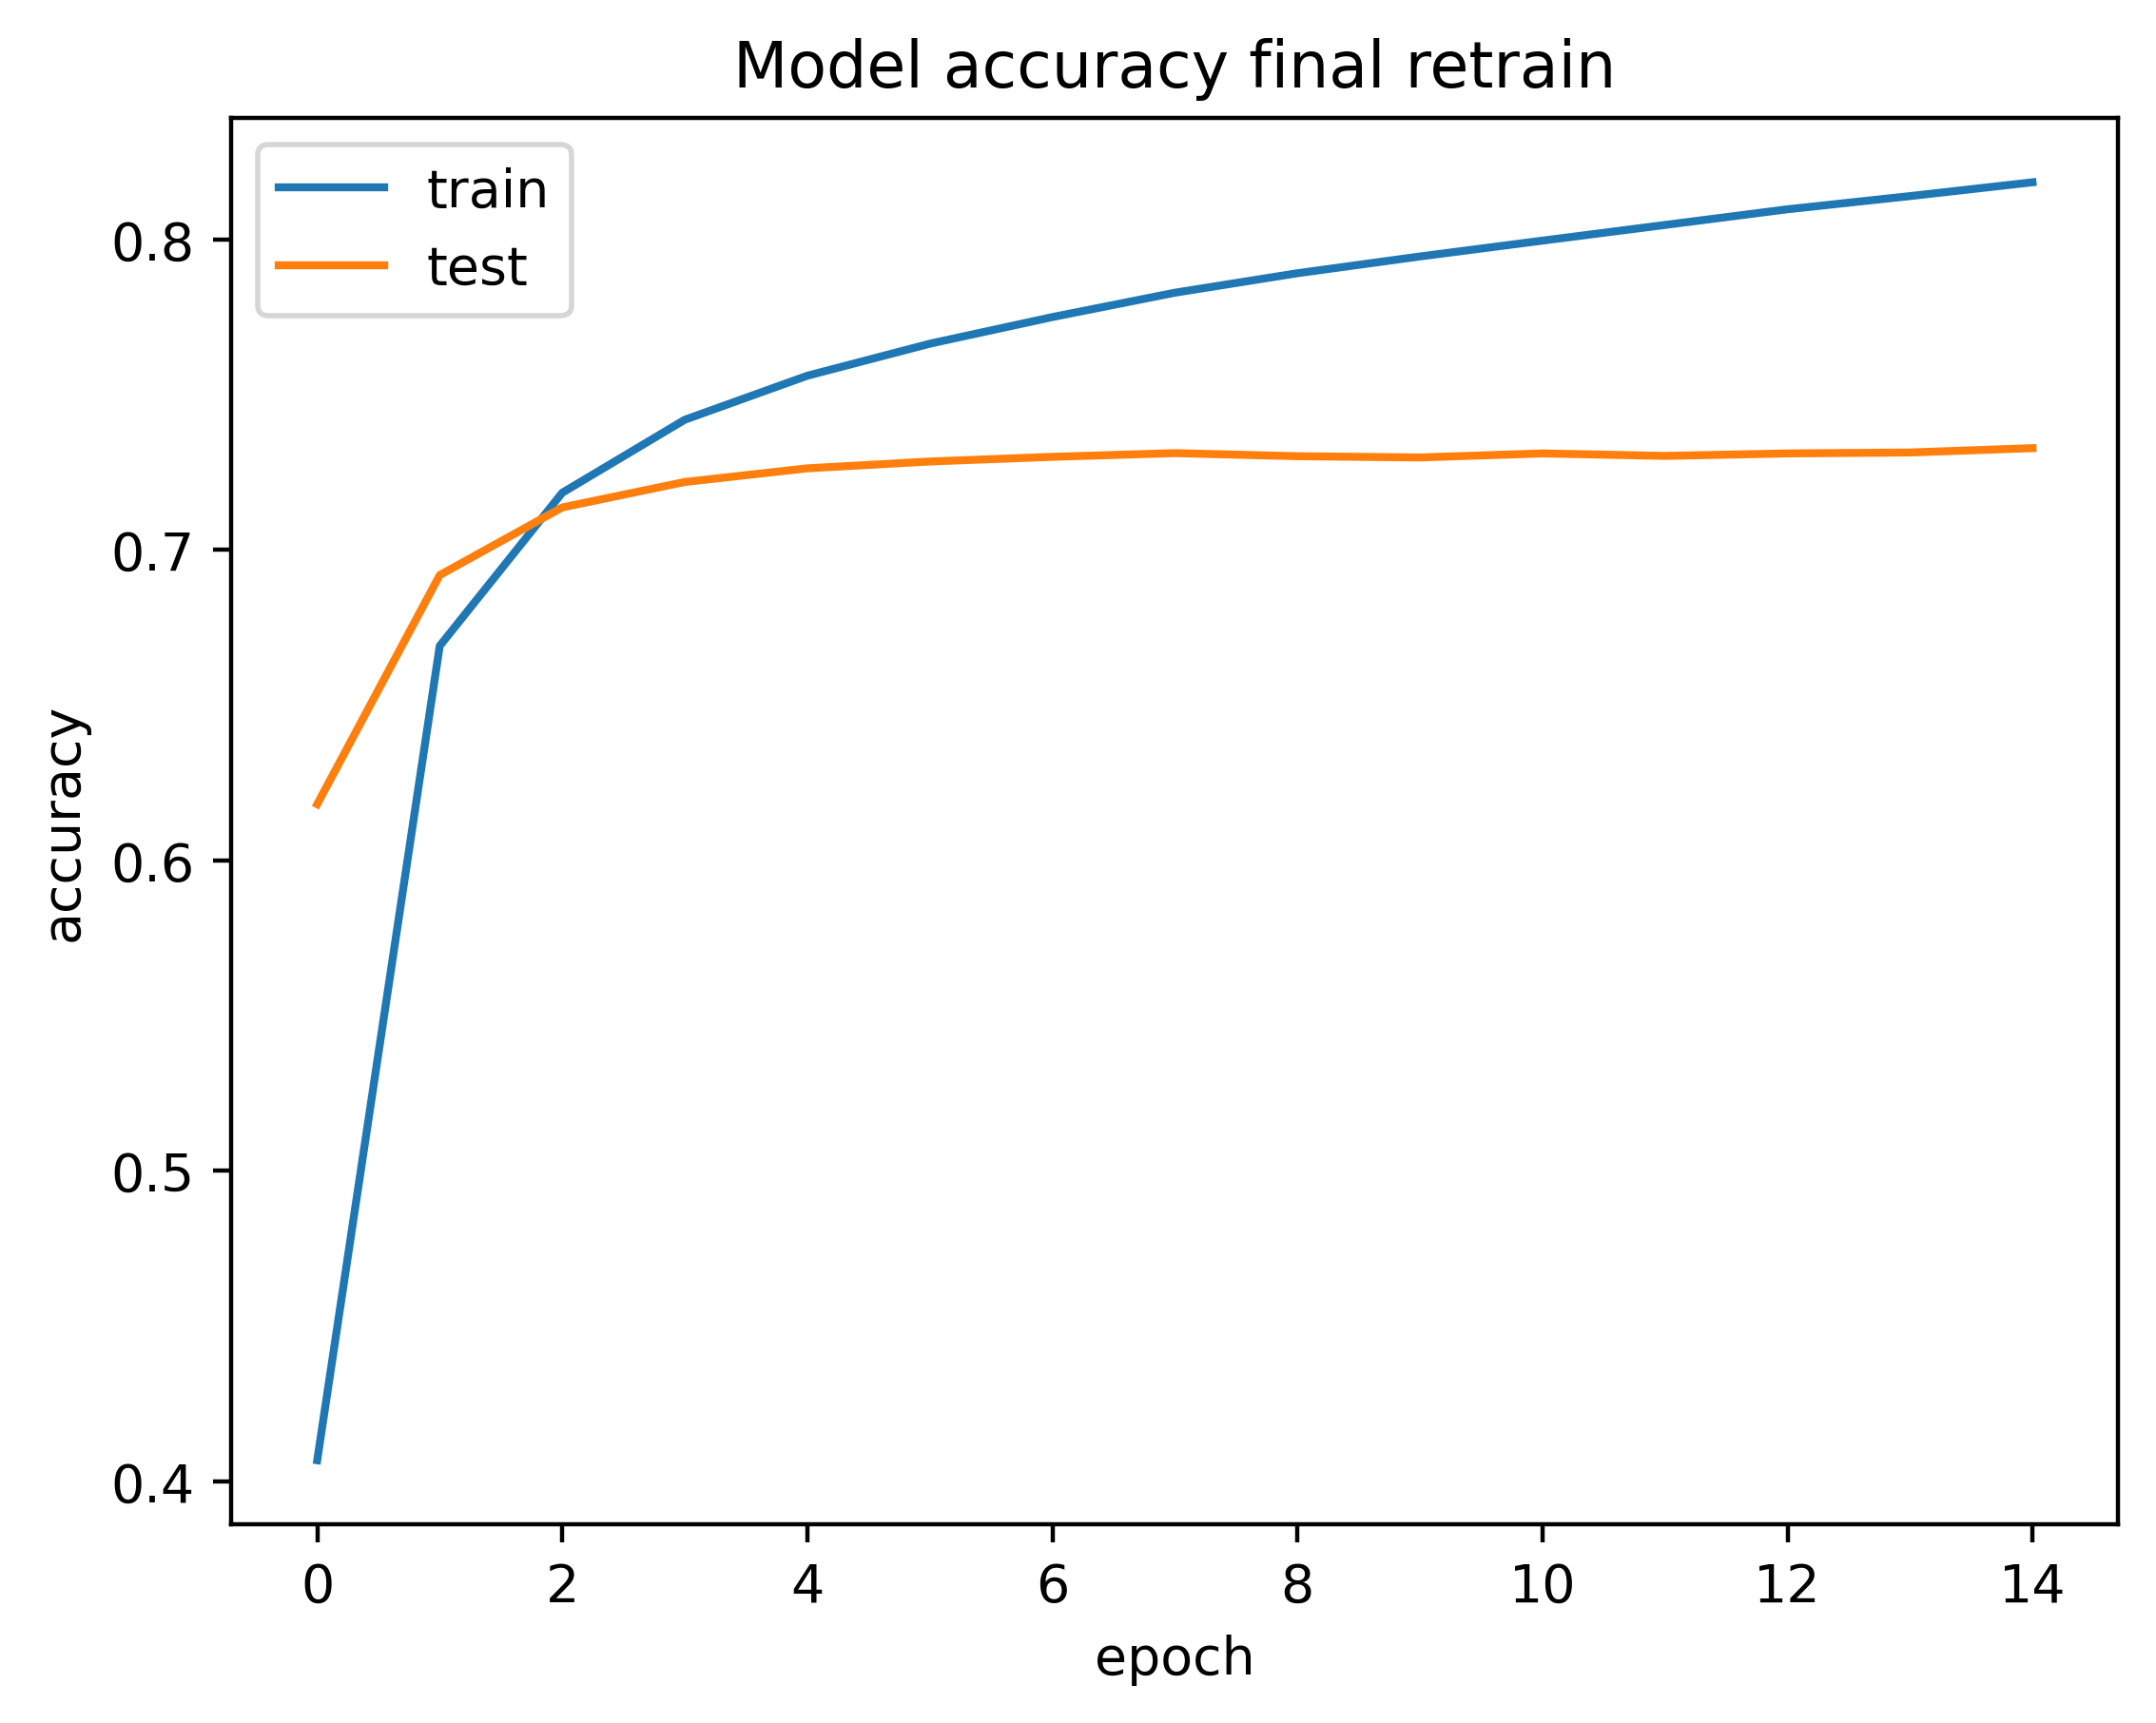
\includegraphics[width=0.5\textwidth,keepaspectratio]{figures/50_final_png_first.png}
\caption{\textit{Accuracy function} após re-treino com o conjunto de treino na totalidade}
\label{diagram:accuracy_retrain}
\centering
\end{center}
\end{figure}

\subsection{Melhoria do modelo}

Para evitar o fenómeno de \textit{overfit}, decidimos acrescentar uma função de regularização nos pesos, \textit{L2 regularization penalty} \cite{l2_regularizer}, nas \textit{hidden layers}. No fundo, a regularização evita o fenómeno de \textit{overfit}, restringindo os valores dos pesos, evitando que o modelo se adapte demasiado à forma dos dados de treino e não consiga generalizar tanto em dados de teste.
Para isso, o algoritmo de regularização tem um parâmetro que define o impacto da regularização nos termos. Caso o valor seja muito elevado, o modelo não tem flexibilidade suficiente para se formatar à forma dos dados, pelo que irá ocorrer o fenómeno de \textit{underfit}. Caso seja muito baixo, o fenómeno de \textit{overfit} pode ocorrer, pois o impacto do termo regularizador é fraco.
Como se pode observar no gráfico \ref{diagram:reg_factor}, para valores muito altos do factor de regularização, o modelo não consegue generalizar os dados. O que acabou por se tornar o melhor parâmetro foi o valor de $0.001$, cuja diferença entre a \textit{accuracy} do conjunto de validação e o conjunto de treino é menor.

Os valores após retreino, usando o factor de regularização óptimo definido acima, são:
\begin{itemize}
        \item \textbf{\textit{Train Score}}: 0.82
        \item \textbf{\textit{Test Score}}: 0.76
\end{itemize}

Como se pode observar no gráfico \ref{diagram:accuracy_retrain_last}, houve uma melhoria relativamente à \textit{accuracy} em dados nunca vistos pelo modelo, o que indica que o fenómeno de \textit{overfit} diminui, o que consequentemente indica que o modelo obteve uma performance melhor.



\begin{figure}[t]
\begin{center}
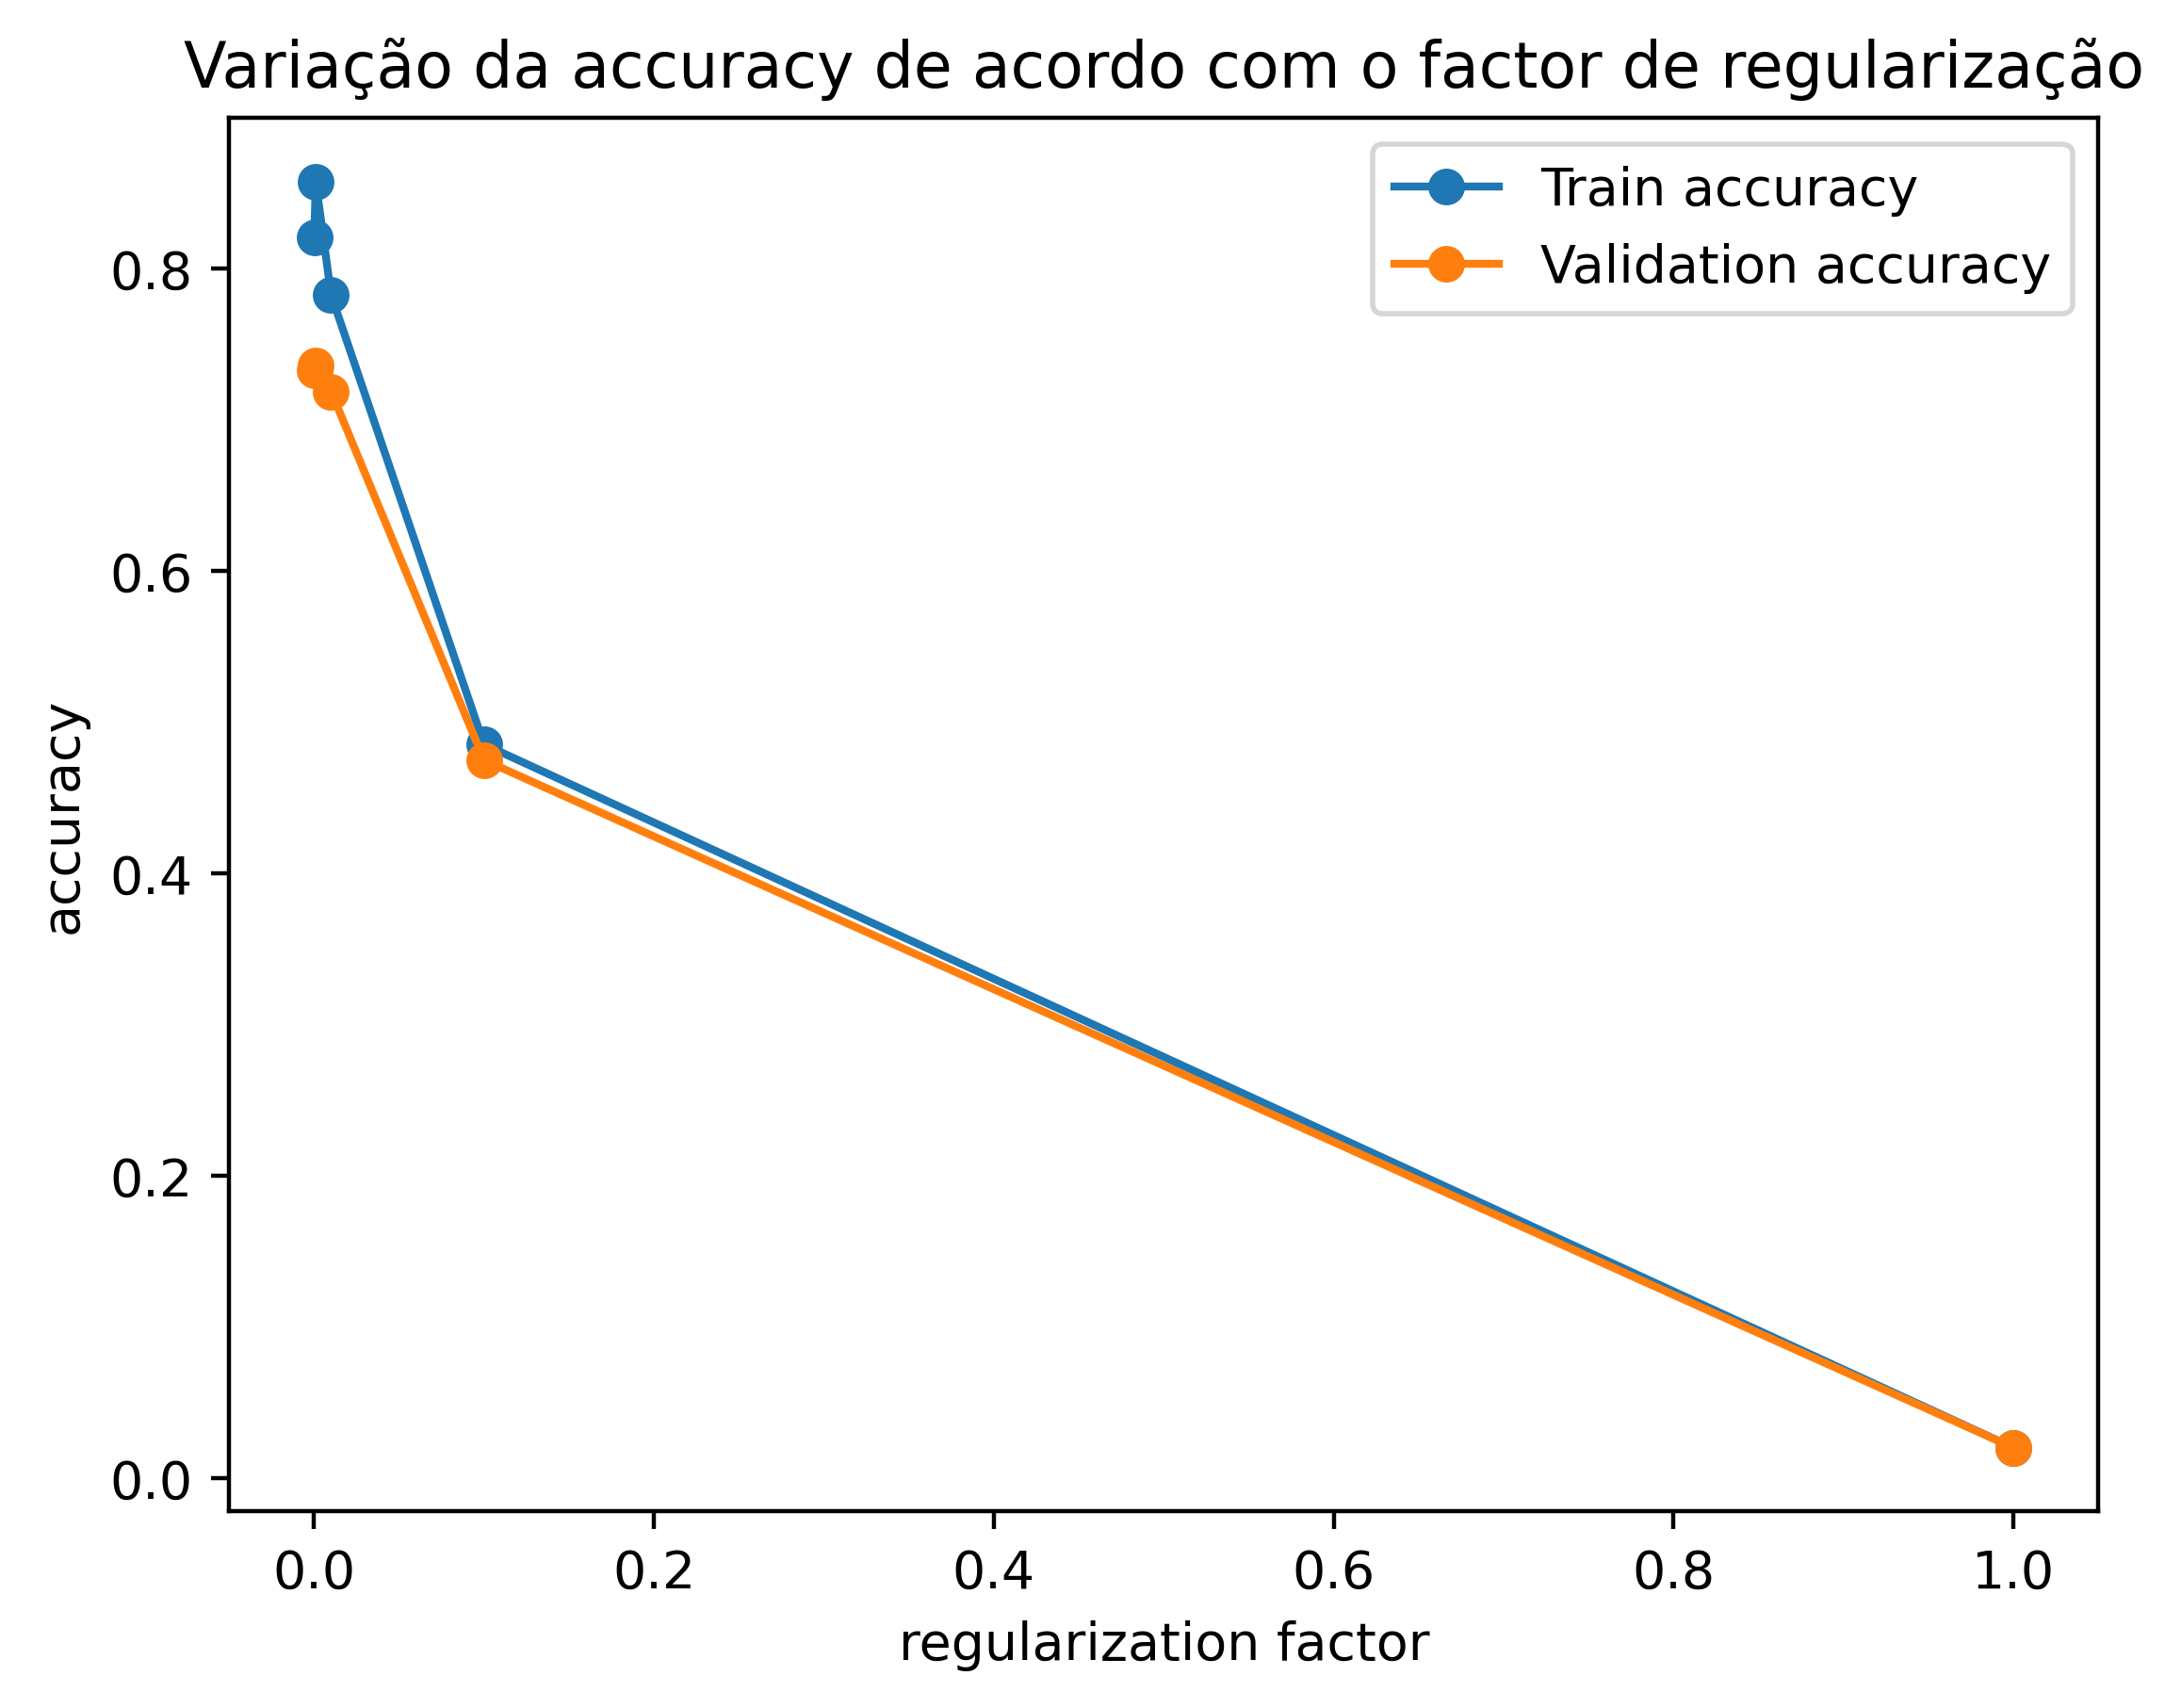
\includegraphics[width=0.5\textwidth,keepaspectratio]{figures/r_Factor.png}
\caption{Variação dos valores de \textit{accuracy} de acordo com o factor de regularização}
\label{diagram:reg_factor}
\centering
\end{center}
\end{figure}


\begin{figure}[t]
\begin{center}
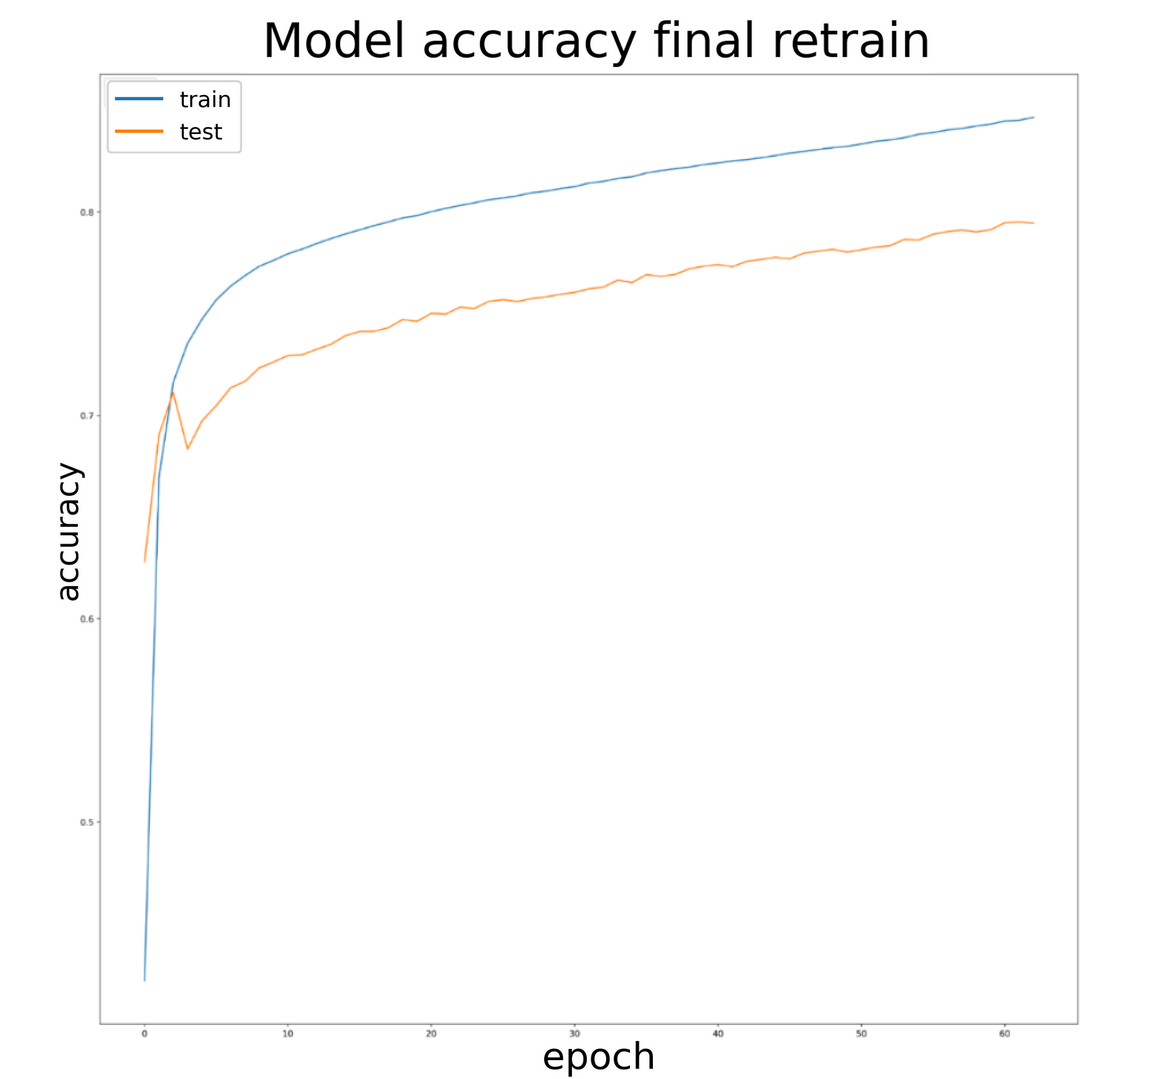
\includegraphics[width=0.5\textwidth,keepaspectratio]{figures/last_retrain_better.png}
\caption{\textit{Accuracy function} após re-treino com o conjunto de treino na totalidade}
\label{diagram:accuracy_retrain_last}
\centering
\end{center}
\end{figure}

\subsection{Análise de sentimento como processo de complementação}

Com a análise prévia dos textos fornecidos no \textit{dataset} e com o conhecimento prévio da plataforma \textit{Reddit}, foi observado que os textos têm alguma complexidade e variância no que toca à formalidade do mesmo.
Para facilitar a compreensão de um determinado texto, foi usado um mecanismo capaz de qualificar um texto em positivo,negativo e neutro.

Após alguma pesquisa foi encontrado um repositório publico de uma ferramenta para a finalidade descrita anteriormente - \textbf{VADER Sentiment Analysis} \cite{vader} baseando-se em regras léxicas e semânticas com intuito de retirar a expressão de sentimentos de dados provenientes de redes sociais.

Esta ferramenta aceita como dados de entrada qualquer sequência de termos alfa-numéricos e retorna algumas pontuações. Apesar dos variados valores de retorno foi usado apenas a seguinte pontuação - \textit{compound score}:
\begin{itemize}
    \item \textbf{Sentimento positivo}: pontuação $>=$ 0.05
    \item \textbf{Sentimento neutro}: 3-0.05 $<$ pontuação $<$ 0.05
    \item \textbf{Sentimento negativo}: pontuação $<=$ -0.05
\end{itemize}

Como esta etapa foi usada como processo de complementação, este modelo foi aplicado a todos os textos do \textit{dataset}, com objectivo de mapear um valor capaz de qualificar o sentimento dos textos. Essencialmente, o vector de \textit{features} é composto pelos vectores de pontuações descritos na secção dos dados  \ref{subsub:data_pre_processing} mais a pontuação proveniente do método descrito.

Para efeitos de aprovação, o gráfico \ref{diagram:Sentiment_vs_no_sentiments} apresenta os valores da \textit{accuracy} do mesmo modelo de \textit{Rede Neuronal} já apresentado durante esta secção, com e sem a \textit{feature} que transmite o sentimento do texto. Como se pode observar, o modelo que dispunha da indicação do sentimento de texto obteve uma melhor performance em termos de \textit{accuracy} em ambos os conjuntos, o que indica que este valor é uma boa adição para a performance do modelo, já que ajuda a descodificar a parte semântica do texto que não é observável apenas com a noção de \textit{tokens}.


\begin{figure}[!t]
\begin{center}
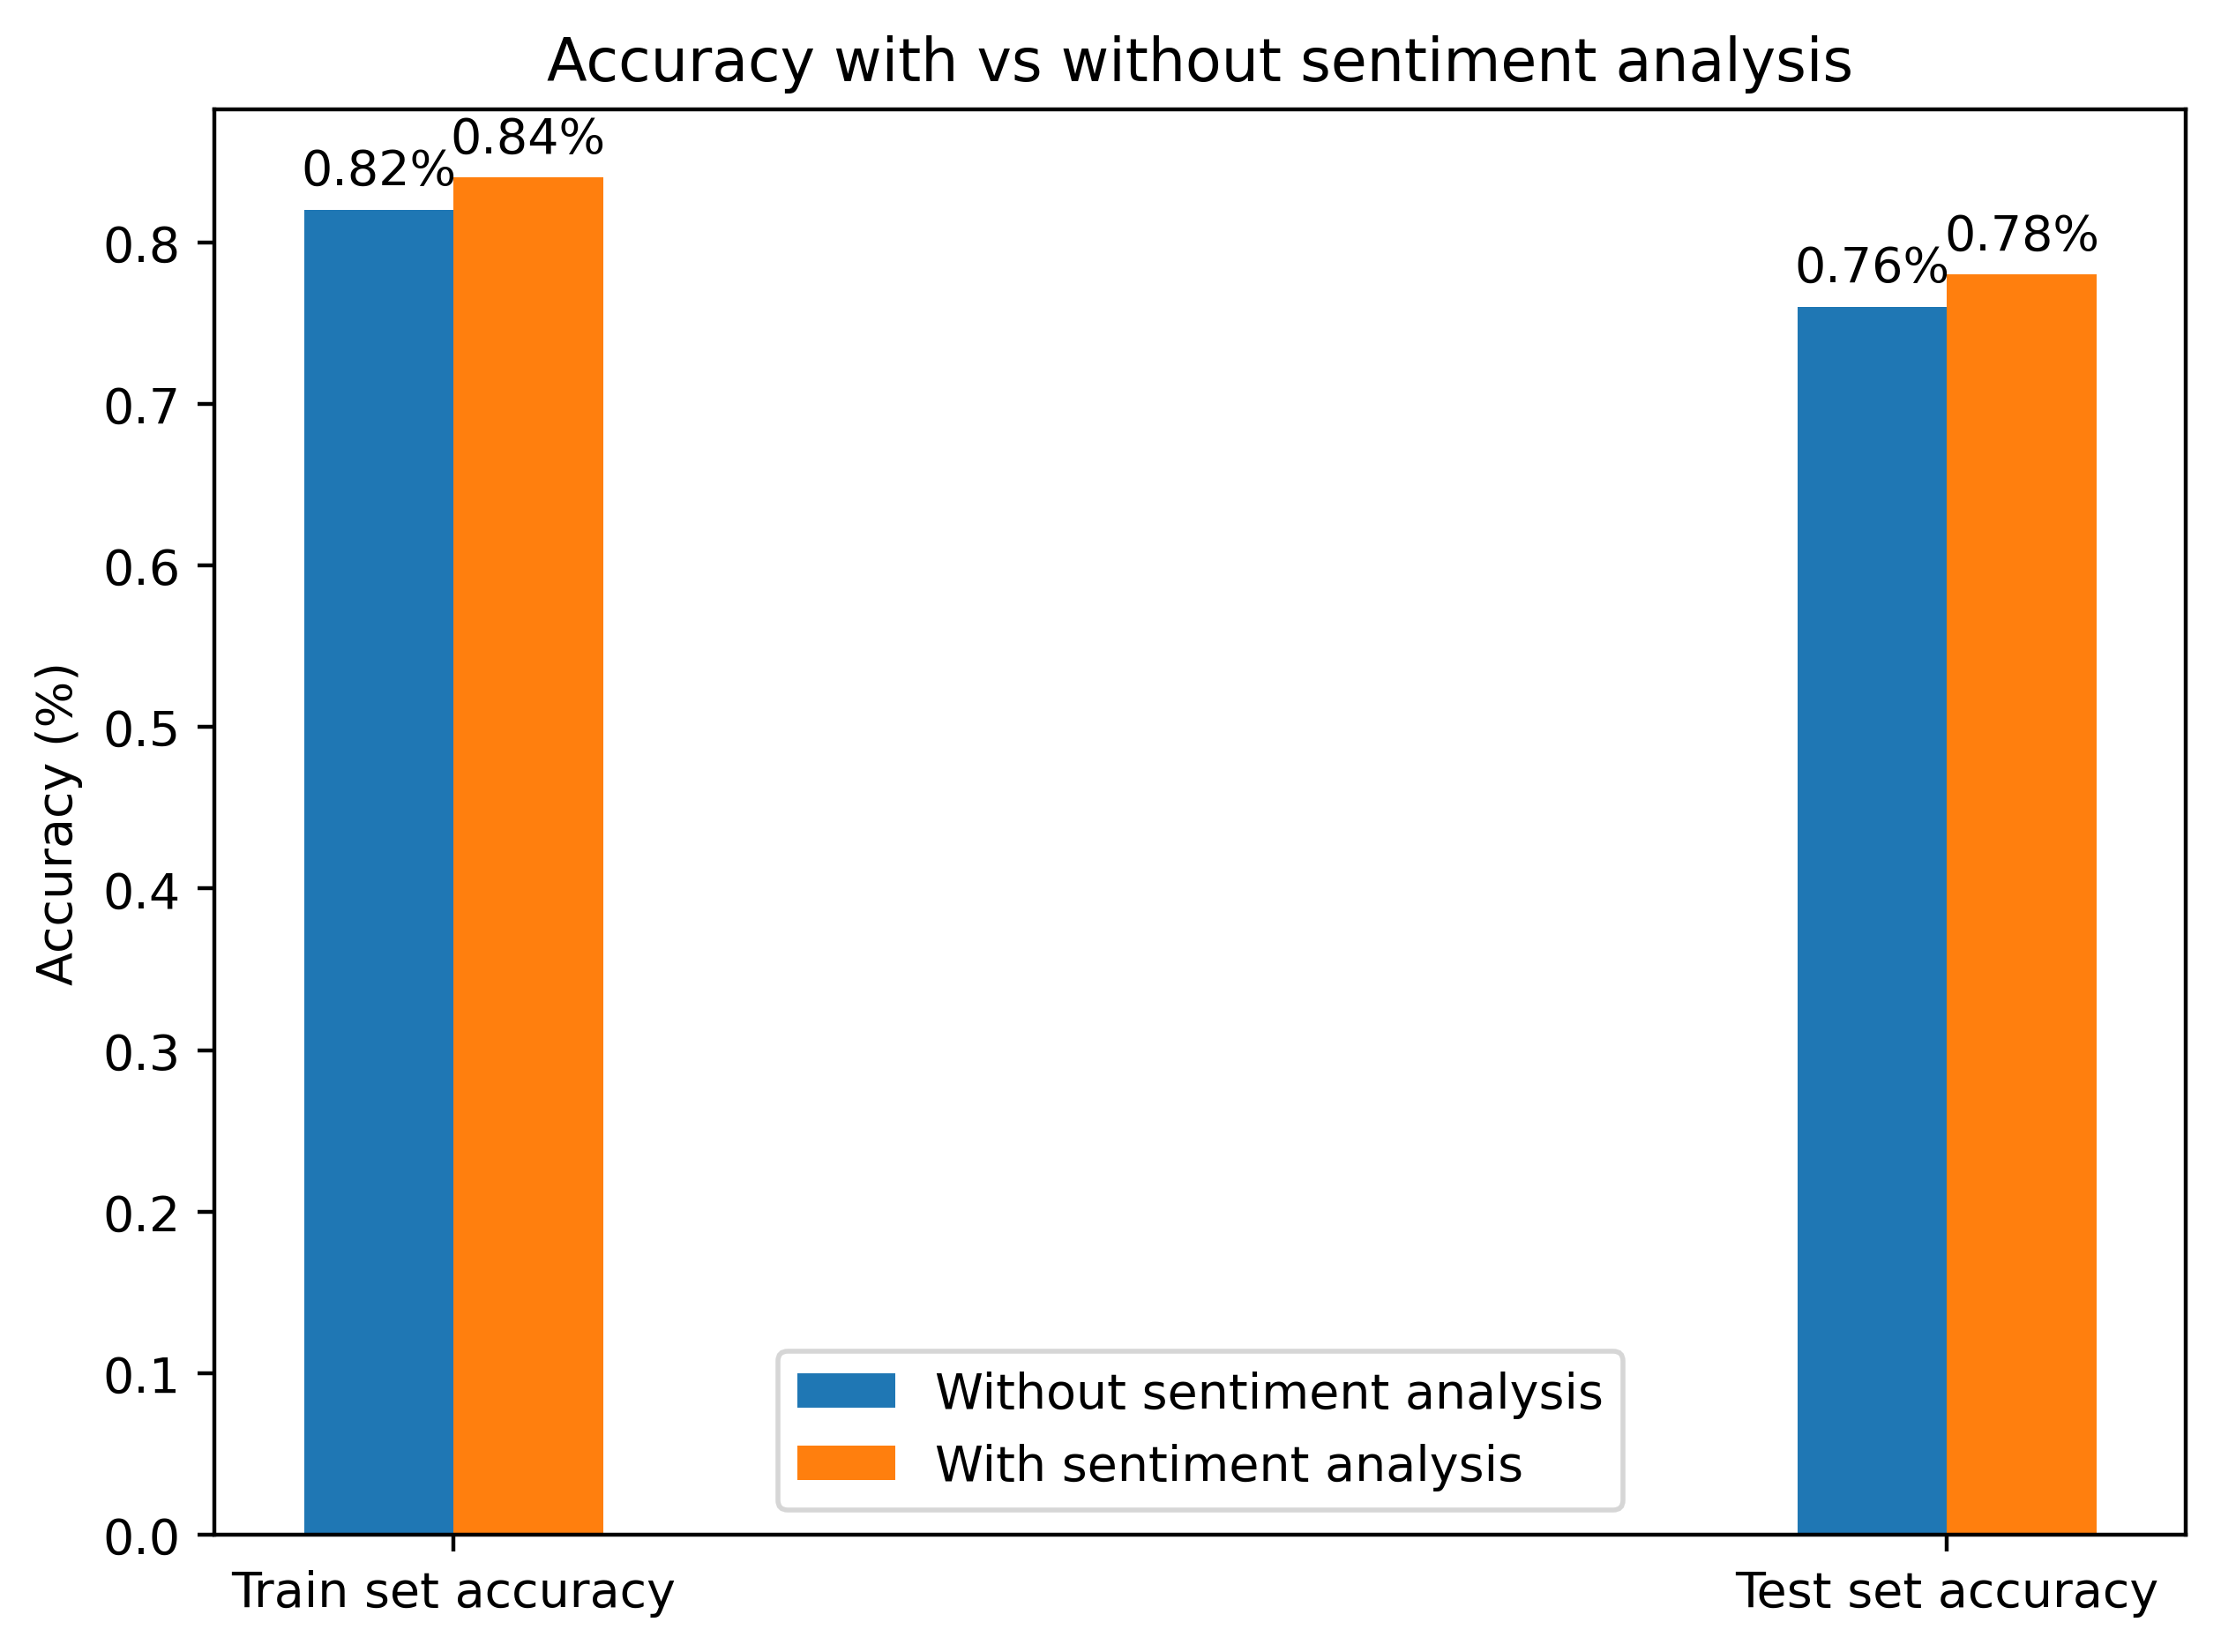
\includegraphics[width=0.5\textwidth,keepaspectratio]{figures/sentiment_vs_no_sentiment.png}
\caption{\textit{Accuracy} do mesmo modelo \textbf{com e sem} o valor que transmite o sentimento do texto}
\label{diagram:Sentiment_vs_no_sentiments}
\centering
\end{center}
\end{figure}



\subsection{Conclusões}
Foram feitos esforços para tentar melhorar a performance deste modelo mas sem sucesso, muito devido à grande dificuldade de \textit{"fine-tune"} das Redes Neuronais, que muito facilmente convergem para o fenómeno de \textit{overfit}.
